\documentclass{article}

\usepackage{amsmath}

\usepackage{graphicx}

\usepackage[dvipsnames]{xcolor}

\begin{document}
	
	**compile and then press F7 for the embedded pdf**
	
\section{Roboat - roboat.org -} 

Roboat is an autonomous boat that is used to realize a responsive, in-demand, infrastructure. The applicatins of Roboat include passenger transportation, garbage collection and package delivery. Additionally units of Roboat can join together to create an on-demand infrastructure such as bridges in water canals. These activities are carried out, as the case with autonomous cars, while simultaneously collecting data about the city. 

\subsection{Features}

\textbf{Obstacle Avoidance}: including navigation and heading with robustness to external environment factors, such as wind and etc. 
\\
\textbf{Automated Docking}: it is able to navigate and latch itself to a docking station via a set of robotic arms (for latching)
\\
\textbf{Different Scales} the system is available in a 1/4 scale, a half-scale and a full-scale 

\subsection{Associated Publications}
\textbf{Robust Place Recognition using an Imaging Lidar, 2021 in IEEE ICRA}:

A rotation invariant method is proposed that leverages 3D point clouds generated from a Lidar. The intensity of the point cloud provided by the lidar is projected and an intensity image is then extracted. ORB features are then extracted from the image and are then encoded into a "bag-of-words" vector using DBoW on a pre-trained visual vocabulary. 
\\
\textcolor{gray}{- To represent an image using BoW "Bag of Words" a document is to be generated form the image, i.e. the image has to somehow be represented as words that will make up the document, three steps are required: feature detection, feature description (or feature representation with stuff like SIFT) and codebook generation BoW can also be defined as a histogram representation based on independent features, for more see the paper:
\\ http://www.cs.nott.ac.uk/~pszqiu/webpages/Papers/ColorPatternRecognition.pdf -}
\\
The vector, used to identify the point cloud, is inserted into a database that is maintained by DBoW for fast place recognition queries and then a returned candidate is thrown. Several techniques such as PnP (Perspective-n-Point)?? and RANSAC are used to minimize the reprojection error of the visual features in 2D image space. Rotation invariance is realised via combining readings from both a Lidar and a camera. An evaluation of the proposed method is carried out on various datasets. 
\\
\textbf{Roboat II: A Novel Autonomous Surface Vessel for Urban Environments, 2020 in EEE/RSJ}
\vspace{3pt}
\\

Roboat II is a novel autonomous surface vessel (ASV), it's used for urban transportation of payloads. It incorporates accurate SLAM, 'Receding Horizon Tracking' using a receding horizon controller\footnote{Receding Horizon (RH) or Model Predictive Control (MPC) is one of the frequently used optimization control techniques in industry. It is designed to handle optimization problems with constraints. It is an online optimization algorithm that predicts system outputs based on current states and system model, finds an open loop control profile by numerical optimization, and applies the first control signal in the optimized control profile to the systems.}. Roboat II is also capable of holonomic motion (i.e. the system doesn't have constraints with regard to its planar motion). 
The SLAM Algorithm receives data from 3 types of sensors, a 3D LiDAR, an IMU and a GPS. To tackle the multi-sensor fusion problem it utilizes a 'factor graph'.

\begin{figure}[htbp]
	\centerline{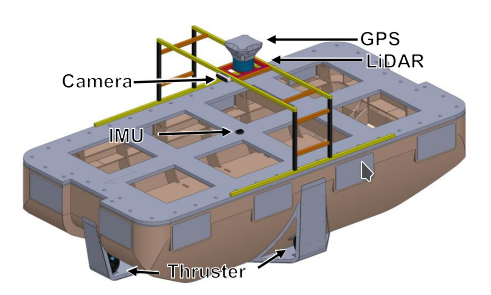
\includegraphics[scale=.5]{roboatII-HW.png}}
	\caption{Roboat II Hardware}
	\label{fig}
\end{figure}

As the dynamics are complex, especially in the water, the system utilizes an online nonlinear model predictive controller (NMPC), the dynamical model is estimated experimentally to achieve satisfactory results regarding the tracking control. 
The state estimation is done simultaneously via a nonlinear moving horizon estimation (NMHE) algorithm. 
The system, according to the authors, is able to perform online mapping and localization (SLAM algorithm gives good results), plan its path and track the planned trajectory. 

\begin{figure}[htbp]
	\centerline{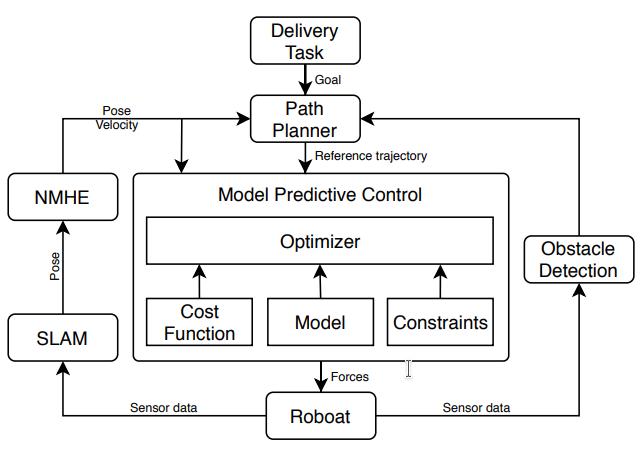
\includegraphics[scale=.5]{roboat-autonomy-framework.png}}
	\caption{autonomy framework of Roboat II. It mainly contains
		a planner, a SLAM module, an NMPC tracking module, an NMHE state
		estimator and a simple object detector.}
	\label{fig2}
\end{figure}


\textbf{An Adaptive Large Neighbourhood Search for Real-Time Waste Collection Inventory Routing with Autonomous Vessels, 2020 in hEart}
\vspace{3pt}
\\
In this paper an inventory system to collect garbage from the water canals in Amsterdam is developed using Adaptive Large Neighborhood Search Algorithm (ALNS), which deals with pick-up and delivery problems. For path planning the $A*$ Algorithm is deployed, which chooses the shortest route from one point to the other through various path points after weighing the cost of each path. 


\section{ClearBot- clearbot.org -} 
ClearBot realizes 3 types of boats for 3 different tasks. It is powered fully by solar energy. The ClearBot types undertake: 
\begin{itemize}
	\item Oil/Trash cleanup
	\item Cargo movement
	\item Foam cleanup, i.e. foam that accumulates in water treatment facilities
\end{itemize}
	


\section{TARMEM (Teams of Aquatic/Aerial Robots for Marine Environment Monitoring) - tarmem.org -} 

The aim of the ongoing project is to develop a team of autonomous robots, consisting of USVs and UAVs, unmanned surface vehicles and unmanned aerial vehicles respectivly to collect and monitor marine data. Up to the point of wiring this and according to the website, only a proof of concept of the system has been developed. \vspace{5pt} \\ 
\textbf{Challenges and how they are solved:}
\begin{itemize}
	\item battery autonomy of UAVs \\
	$\hookrightarrow$ UAVs are carried and can recharge in the corresponding USV
	\item landing and takeoff, especially with weather and marital conditions \\
	$\hookrightarrow$ utilization of a 6 DOF landing platform
	
	\begin{figure}[htbp]
		\centerline{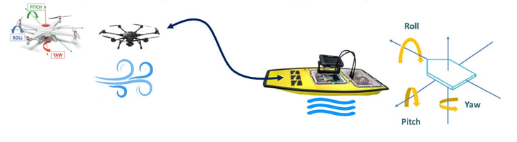
\includegraphics[scale=1]{tarmem-landing.png}}
		\caption{landing on the USV platform}
		\label{fig3}
	\end{figure}

\begin{figure}[htbp]
	\centerline{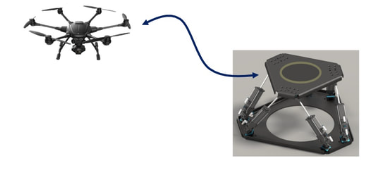
\includegraphics[scale=1]{tarmem-landing-platform.png}}
	\caption{6 DOF platform for landing}
	\label{fig4}
\end{figure}
	
	\item schedule, rendez-vous between the UAV and USV \\
	$\hookrightarrow$ model the problem as a dynamic TSP with uncertainty that is solved online using a robust optimisation approach
	\item coordination regarding: assigning collision-free trajectories -- division of monitoring and/or data collection area \\
	$\hookrightarrow$ \textbf{developing a novel approaches for non-holonomic navigation control under disturbances (combination of integer optimization and auction based models for decentralized planning and adaptive replanning, swarm intelligence for coalition information)}
	\item wireless communication considering the lack of high-bandwidth in open waters \\
	$\hookrightarrow$ multi-hop ad hoc networking 
	\item autonomy robustness with regard to harsh marital conditions \\
	$\hookrightarrow$ system level assessment of weather conditions and resilient patter formation  
	
	\begin{figure}[htbp]
		\centerline{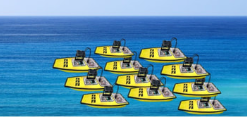
\includegraphics[scale=1]{tarmem-pattern-formation.png}}
		\caption{TARMEM pattern formation}
		\label{fig5}
	\end{figure}
	
\end{itemize} 

\subsection{Associated Publications https://www.tarmem.org/publications.html}




\section{Websites}

roboat.org \\
clearbot.org \\
tarmem.org \\
mas400.com \\
oceanalpha.com \\
Clean Path Robotics- Heron USV

\end{document}